\documentclass{article}
% \usepackage[utf8x]{inputenc}
\usepackage{microtype}
%\usepackage[icelandic]{babel}


\usepackage[T1]{fontenc}
\usepackage[utf8]{inputenc}
\usepackage{lmodern}

\usepackage{verbatim}
\usepackage{booktabs}
\usepackage{graphicx}
\usepackage{amsmath}
\usepackage{tcolorbox}
\usepackage{subcaption}
\usepackage{hyperref}
\usepackage[margin=3cm]{geometry}


% Default fixed font does not support bold face
\DeclareFixedFont{\ttb}{T1}{txtt}{bx}{n}{12} % for bold
\DeclareFixedFont{\ttm}{T1}{txtt}{m}{n}{12}  % for normalf

% Custom colors
\usepackage{color}
\definecolor{deepblues}{rgb}{0,0,0.5}
\definecolor{deepred}{rgb}{0.6,0,0}
\definecolor{deepgreen}{rgb}{0,0.5,0}

\usepackage{listings}

% Python style for highlighting
\newcommand\pythonstyle{\lstset{
language=Python,
basicstyle=\ttm,
otherkeywords={self},             % Add keywords here
keywordstyle=\ttb\color{deepblue},
emph={MyClass,__init__},          % Custom highlighting
emphstyle=\ttb\color{deepred},    % Custom highlighting style
stringstyle=\color{deepgreen},
frame=tb,                         % Any extra options here
showstringspaces=false            %
}}

% Python environment
\lstnewenvironment{python}[1][]
{
\pythonstyle
\lstset{#1}
}
{}

% Python for external files
\newcommand\pythonexternal[2][]{{
\pythonstyle
\lstinputlisting[#1]{#2}}}

% Python for inline
\newcommand\pythoninline[1]{{\pythonstyle\lstinline!#1!}}



\setlength{\columnsep}{1cm}
\setlength\parindent{0pt}

\title{Synthesis of Face Images Using Generative Algorithms.}

\author{René Haas \\ Supervisor: Stella Grasshof}



\begin{document}

\maketitle
\tableofcontents
\newpage


\section{Introduction}

A distinction between machine learning models are that between \emph{disciminative} and \emph{generative} models. In discriminative models we assign a label to a datapoint. For example given an image, which category does it belong to - is it a cat or a horse? Generative models however tries to approximate samples from a data distribution from a learned distribution.

In this research project we will explore different generative models on the domain of face synthesis. We can distinguish two main types of generative models: likelihood based models, which include Variational Autoencoders (VAEs) and implicit models such as Generative Adversarial Networks (GANs)\cite{vqvae2}.

In this project we will implement Principal Component Analysis(PCA) a VAE and a GAN and compare the results of generating faces with these three methods.

We will start in the next
exploring different architectural implementation along the way.

The expected outcome of theis project is theree folde

1) gaining an overview of modern generative models trhough a literature survery. Here we will review recent litterature and explore there different recent  architectural implementation of VAEs and GANS. We will provide the nessecary theory along the way. Wwith we will do in the next section

2) gain practical understanding by implementing versions of the different models and training them two different datasets.

3) Finally we will Furthermore we will explore the latent space of pre trained models and show that we can use these to do state-of-the-art face synthesis and semantic face editing.

\chapter{Theory}


\section{Inception Score}
\url{https://machinelearningmastery.com/how-to-implement-the-inception-score-from-scratch-for-evaluating-generated-images/}


\section{Principal Component Analasyis. }

\section{Probabilistic models}
We assume that the observed variable $\mathbf{x}$ is a sample from the true distribution $p^*(\mathbf{x})$.\cite{vaeintro} Out goal is to approximate the true distribution with a model such that

\begin{align}
  p_\theta(\mathbf{x})\approx p^*(\mathbf{x})
\end{align}

Now, how do we ego about actually modeling this distribution $p_\theta(\mathbf{x})$?. We can use Neural networks to parametrize the distribution.

The log-probability of the data is
\begin{align}
  \log p_\theta(\mathcal{X}) = \sum_{\mathbf{x}\in\mathcal{X}} p_\theta(\mathbf{x})
\end{align}

Maximization of the log-likelihood is equivalent to minimizing the KullBack-Leibler divergence.

The KullBack-Leibler divergence is given by

\begin{align}
D_{\text{KL}}(p_\theta,q_\phi) = -\sum_{\mathbf{x}\in\mathcal{X}}p_\theta(\mathbf{x})\log \frac{q_\phi(\mathbf{x})}{p_\theta(\mathbf{x})}
\end{align}

% \section{Survey}

\section{Variational Autoencoders.}
The encoder network models$p_\theta(\mathbf{z}|\mathbf{x})$ while the encoder network models $p_\theta(\mathbf{x}|\mathbf{z})$


\section{GANs}

The premise of GANs is to play minmax game between two competing neural networks. We simultaneously train a discriminator $D$ and a generator $G$.
The discriminator $D$ is a binary classifier whose objective is classify whether a show example image is coming from the data distribution $p_D$ or from the generated $p_G$ distribution.

The original value function,proposed in 2014 by Ian Goodfellow et al.\cite{gan} is given by
\begin{align}
\mathcal{L} = \min_G \max_D V(D,G))=\mathbb{E}_{\mathbf{x}\sim p_{\text{data}}(\mathbf{x})}
\left[\log D(\mathbf(x))]\right]+
\mathbb{E}_{\mathbf{z}\sim p_{\mathbf{z}}(\mathbf{z})}
\left[\log (1-D(G(\mathbf(z)))]\right]
\end{align}
Here the $G$ tries to minimize $\mathcal{L}$ while the $D$ tries to maximize it.

Since $D$ is taking a data point (image) $\mathbf{x}\in X$ and giving the probability that image is real or generated, it is a mapping $D:X \to (0,1)$.

We define the generator as to depend on a latent variable $\mathcal{z}\in Z$ such that $G(\mathcal{z})$ is a mapping $G:Z\to X$.




% \paragraph{Face Aging}
% \textit{Face Aging With Conditional Generative Adversarial Networks} (2017) \cite{faceaging}

% \section{3D Reconstruction}
%
% \textit{Projective Structure from Facial Motion}(2017)\cite{ProjectiveStructure}
%
% \textit{Apathy is the Root of all Expressions}(2017)\cite{apathy}
%
% In the paper \textit{"Large Pose 3D Face Reconstruction from a Single Image via Direct Volumetric CNN Regression"}(2017)\cite{largepose}
% the authors used a Convolutional Neural Network to reconstruct the 3D facial geometry from just a single image. The model work under arbitrary poses
% and expressions and without the need of a 3D Morphable Model.

\chapter{Results}

\section{Data sets}
In the following we will use two different datasets

\begin{figure}
    \centering
    \begin{subfigure}[b]{0.45\textwidth}
        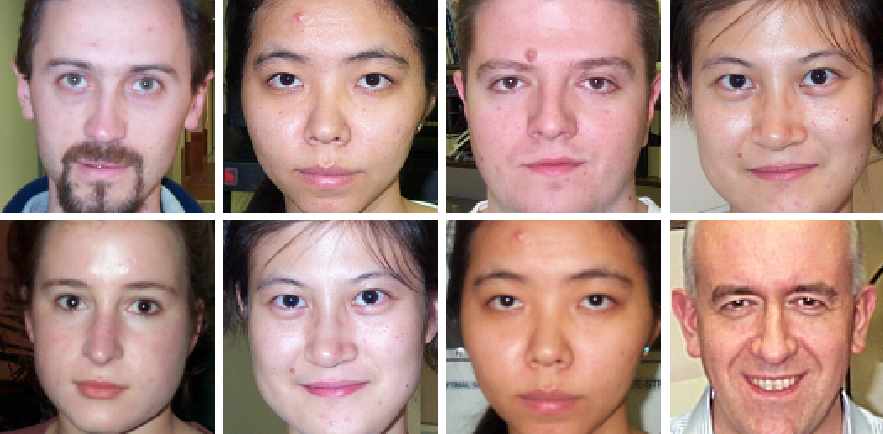
\includegraphics[width=\textwidth]{fig/data/caltech}
        \caption{ Caltech dataset}
    \end{subfigure}
    ~
    \begin{subfigure}[b]{0.45\textwidth}
        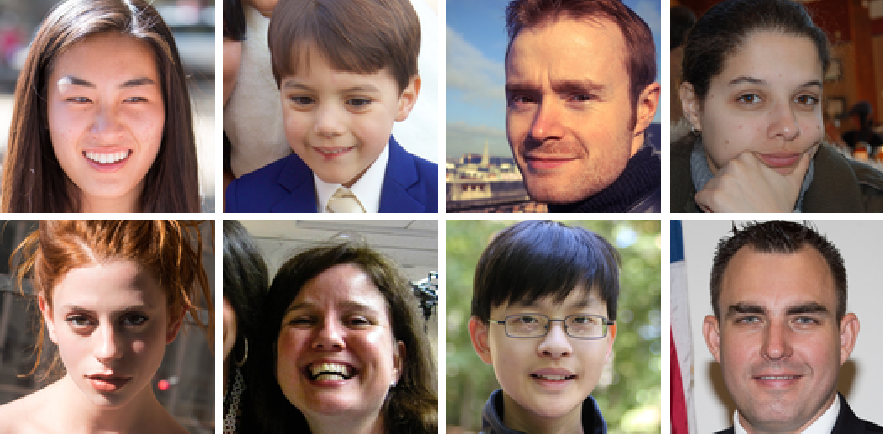
\includegraphics[width=\textwidth]{fig/data/ffhq}
        \caption{FFHQ dataset}
    \end{subfigure}

    \caption{The raw data from the Caltech and FFHQ datasets respectively. This figure is the only one containing images of real people in the report.}
    \label{rawdata}
\end{figure}


\section{Principal Component Analysis }
In this section we explore the results of using Principal Component Analysis (PCA) for face synthesis. PCA is predominately used for dimensionality reduction but here we will use it for synthesis.

The goal of PCA is to find the Principal Components which are the directions of greatest variance in the dataset. These directions are the eigenvectors or, in this context, eigenfaces of the covariance matrix.

Let $\tilde{\mathbf{X}} = \mathbf{X} - \bar{\mathbf{X}}$ then $\mathbf{X}^T\mathbf{X}$ is the covariance matrix we find the eigenfaces the usual way by demanding that $\det(\mathbf{X}^T\mathbf{X} - \lambda) = 0$
We then sort the eigenface after eigenvalue $\lambda$ in order of descending variance. In Figure \ref{eigenface} we see the first 8 eigenfaces.

\begin{figure}
  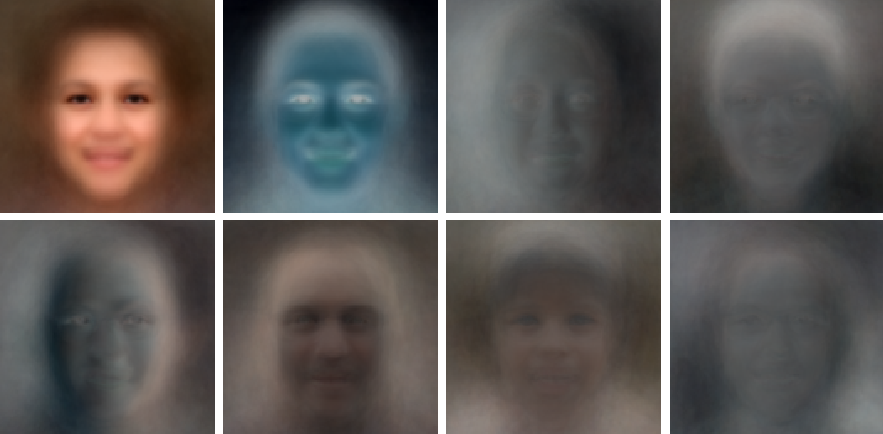
\includegraphics[width=\textwidth]{fig/PCA/pca}
  \caption{Eigenfaces of the FFHQ dataset.}
  \label{eigenface}
\end{figure}

We can generate new synthetic faces $F$ by adding a linear combination of the
eigenfaces $F_i$ to the mean face $F_m$.

\begin{align}
F  = F_m + \sum_{i} \alpha_i F_i
\end{align}
in Figure \ref{pca-components} we see the results of varying the first six
principal components.

In order it seems that the Principal Component control aspects of 1) and 2) Color 3) direction of lighting 4) age 5) pose and 6) gender.


\begin{figure}
    \centering
    \begin{subfigure}[b]{\textwidth}
        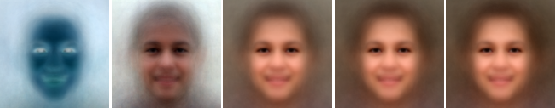
\includegraphics[width=\textwidth]{fig/PCA/pca0}
        \caption{First Principal Component}
    \end{subfigure}
    \begin{subfigure}[b]{\textwidth}
        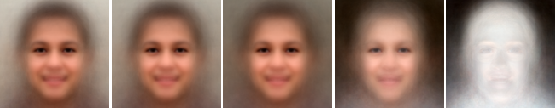
\includegraphics[width=\textwidth]{fig/PCA/pca1}
        \caption{Second Principal Component}
    \end{subfigure}
    \begin{subfigure}[b]{\textwidth}
        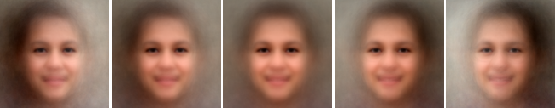
\includegraphics[width=\textwidth]{fig/PCA/pca2}
        \caption{Third Principal Component}
    \end{subfigure}
    \begin{subfigure}[b]{\textwidth}
        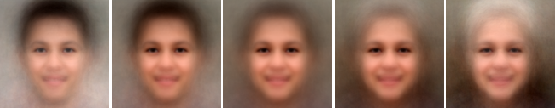
\includegraphics[width=\textwidth]{fig/PCA/pca3}
        \caption{Fourth Principal Component}
    \end{subfigure}
    \begin{subfigure}[b]{\textwidth}
        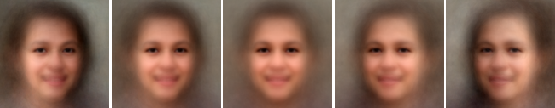
\includegraphics[width=\textwidth]{fig/PCA/pca4}
        \caption{Fifth Principal Component}
    \end{subfigure}
    \begin{subfigure}[b]{\textwidth}
        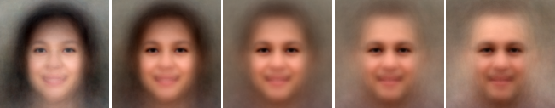
\includegraphics[width=\textwidth]{fig/PCA/pca5}
        \caption{Sixth Principal Component}
    \end{subfigure}
    \caption{Synthetic faces created by varying a single principal component to the mean face.}
    \label{pca-components}
\end{figure}

\section{DCGAN}


\begin{figure}
    \centering
    \begin{subfigure}[b]{0.45\textwidth}
        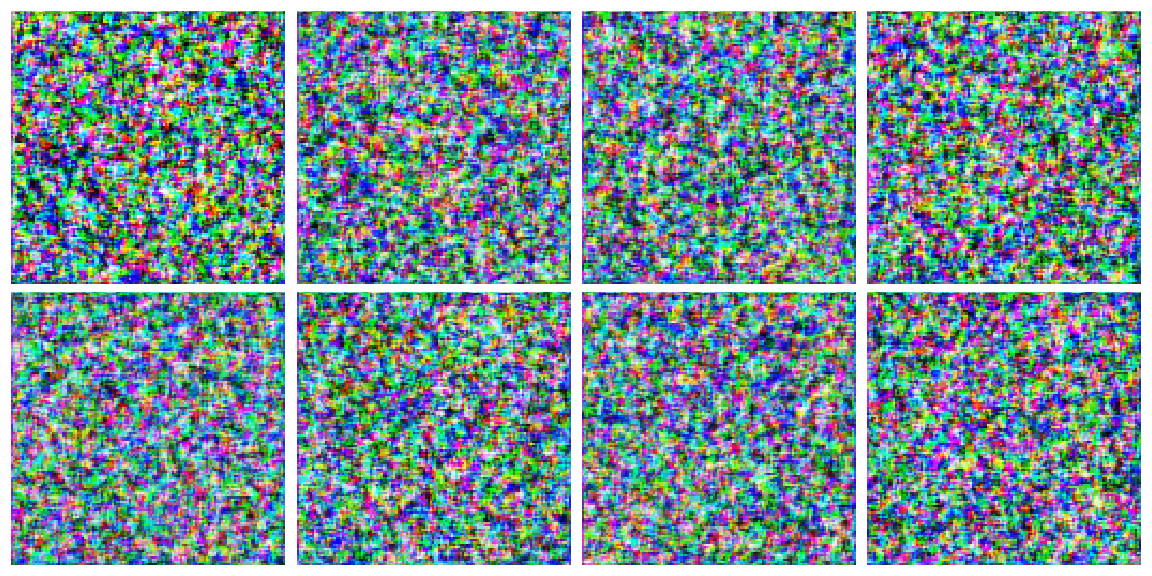
\includegraphics[width=\textwidth]{fig/dcgan/ffhq/epoch0}
        \caption{Epoch 0}
    \end{subfigure}
    ~
    \begin{subfigure}[b]{0.45\textwidth}
        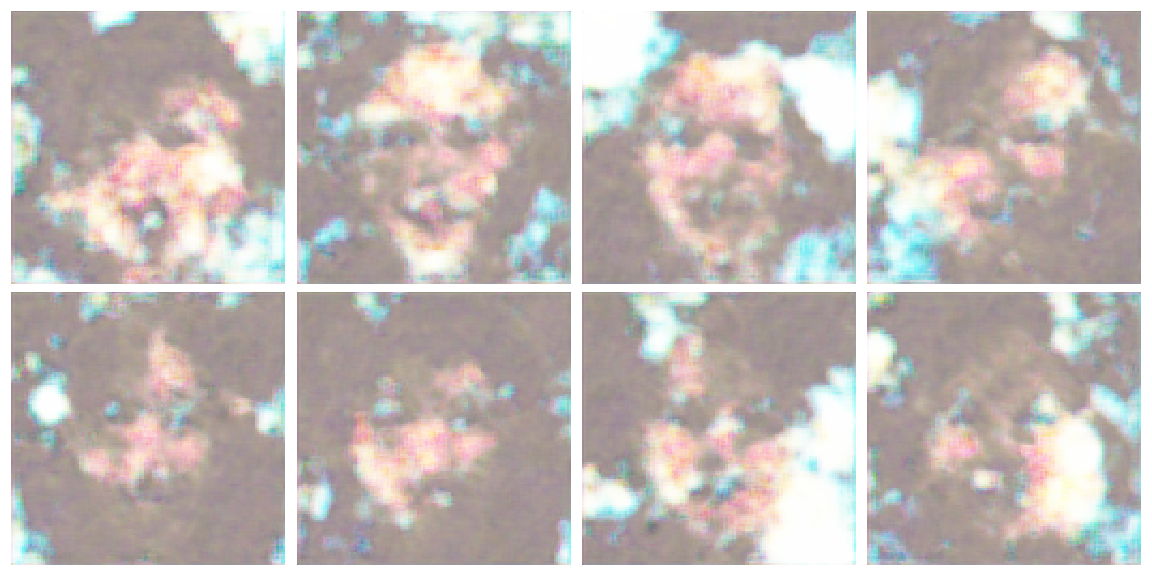
\includegraphics[width=\textwidth]{fig/dcgan/ffhq/epoch200}
        \caption{Epoch 10}
    \end{subfigure}

    \begin{subfigure}[b]{0.45\textwidth}
        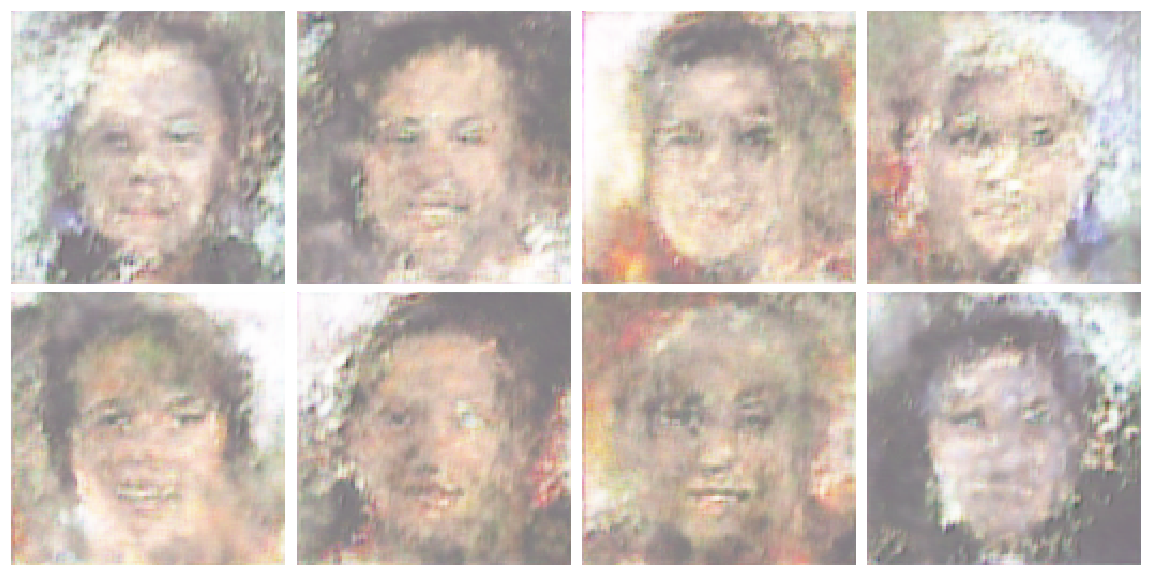
\includegraphics[width=\textwidth]{fig/dcgan/ffhq/epoch2000}
        \caption{Epoch 200}
    \end{subfigure}
    ~
    \begin{subfigure}[b]{0.45\textwidth}
        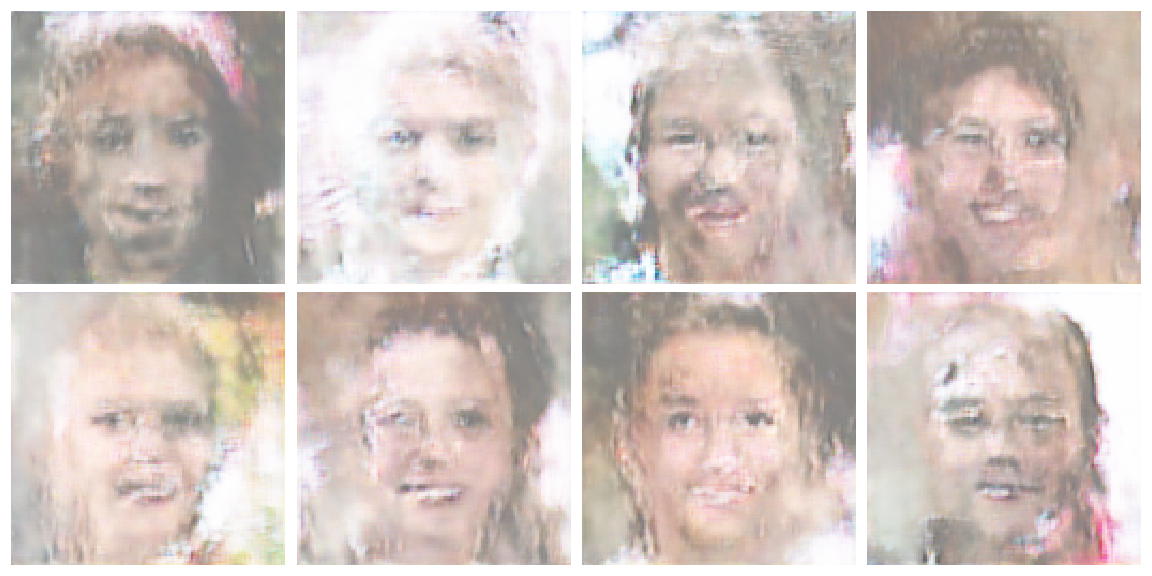
\includegraphics[width=\textwidth]{fig/dcgan/ffhq/epoch4000}
        \caption{Epoch 400}
    \end{subfigure}

    \begin{subfigure}[b]{\textwidth}
        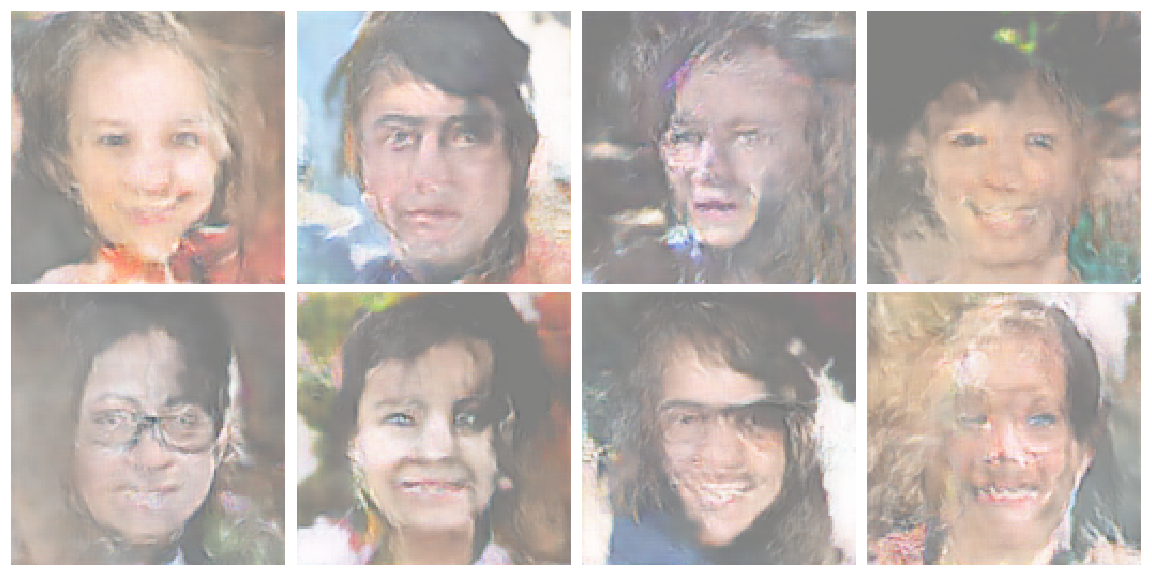
\includegraphics[width=\textwidth]{fig/dcgan/ffhq/epoch10000}
        \caption{Epoch 400}
    \end{subfigure}
    \caption{Samples from DCGAN during training on the FFHQ dataset}
    \label{dcgan-ffhq-samples}
\end{figure}

\begin{figure}

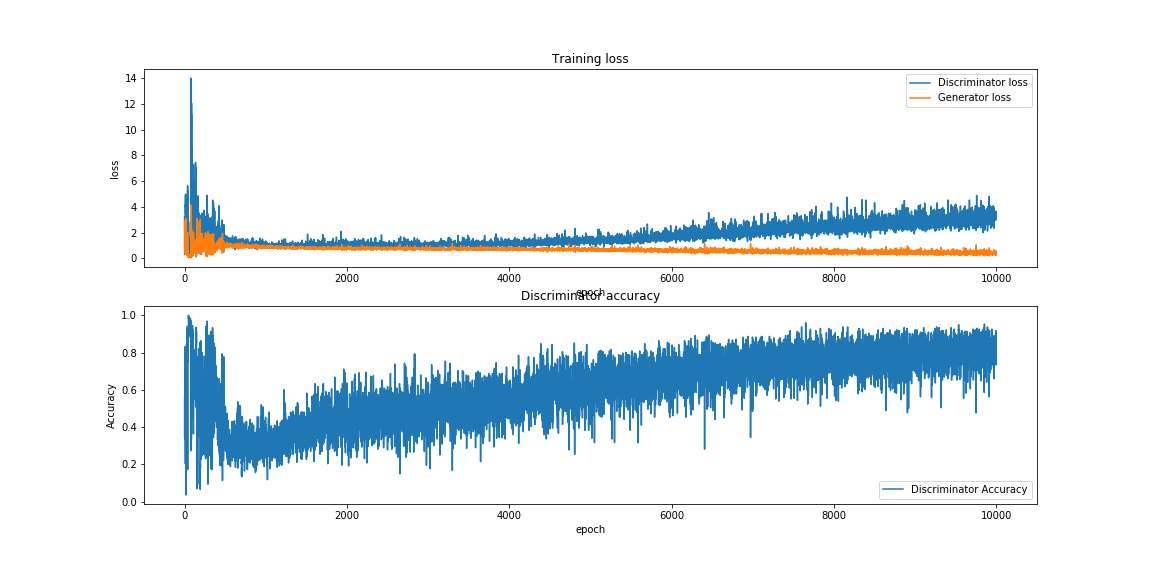
\includegraphics[width=\textwidth]{fig/dcgan/ffhq/loss}
  \caption{Loss and accuracy of the discriminator during training on the FFHQ Datase}
  \label{dcgan-ffhq-loss}
\end{figure}

\begin{figure}
    \centering
    \begin{subfigure}[b]{0.45\textwidth}
        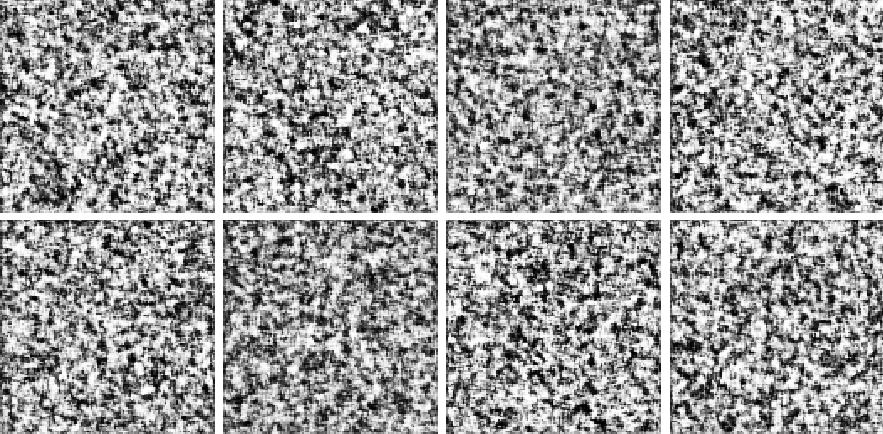
\includegraphics[width=\textwidth]{fig/dcgan/caltech/epoch0}
        \caption{Epoch 0}
    \end{subfigure}
    ~
    \begin{subfigure}[b]{0.45\textwidth}
        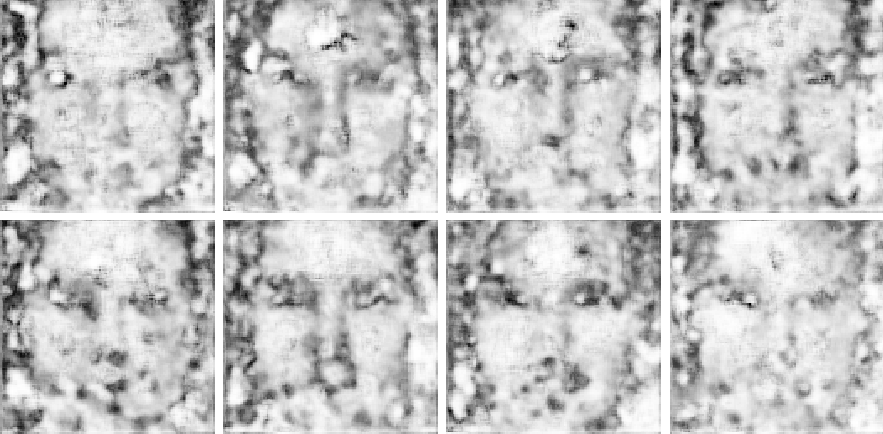
\includegraphics[width=\textwidth]{fig/dcgan/caltech/epoch200}
        \caption{Epoch 10}
    \end{subfigure}

    \begin{subfigure}[b]{0.45\textwidth}
        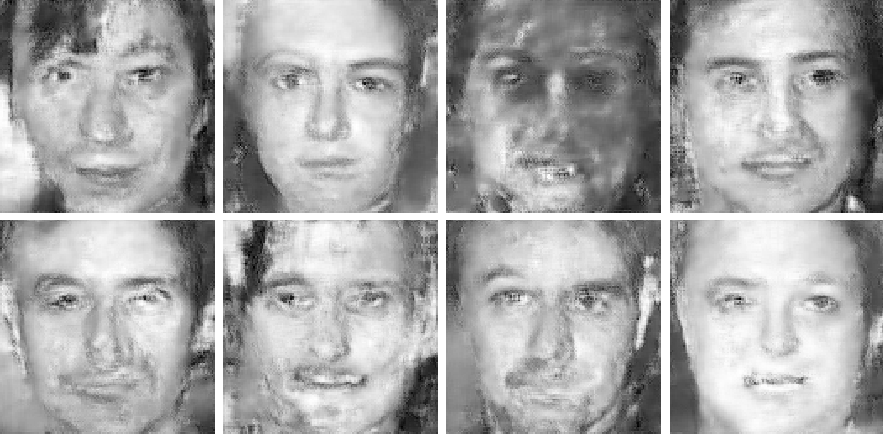
\includegraphics[width=\textwidth]{fig/dcgan/caltech/epoch2000}
        \caption{Epoch 200}
    \end{subfigure}
    ~
    \begin{subfigure}[b]{0.45\textwidth}
        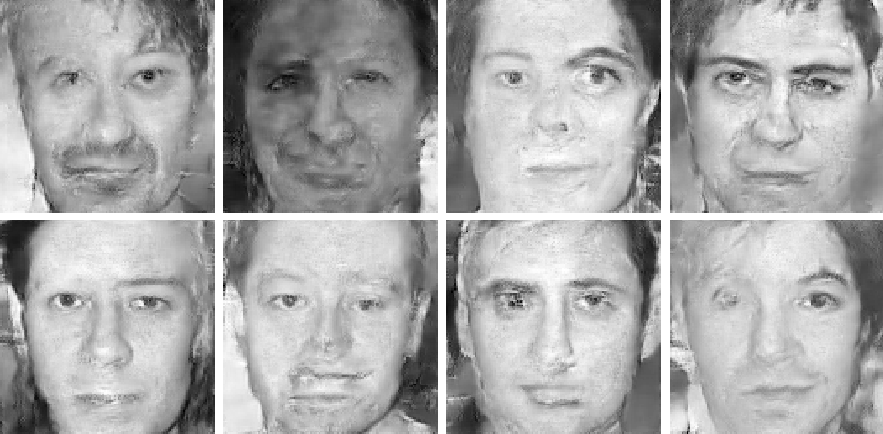
\includegraphics[width=\textwidth]{fig/dcgan/caltech/epoch4000}
        \caption{Epoch 400}
    \end{subfigure}

    \begin{subfigure}[b]{\textwidth}
        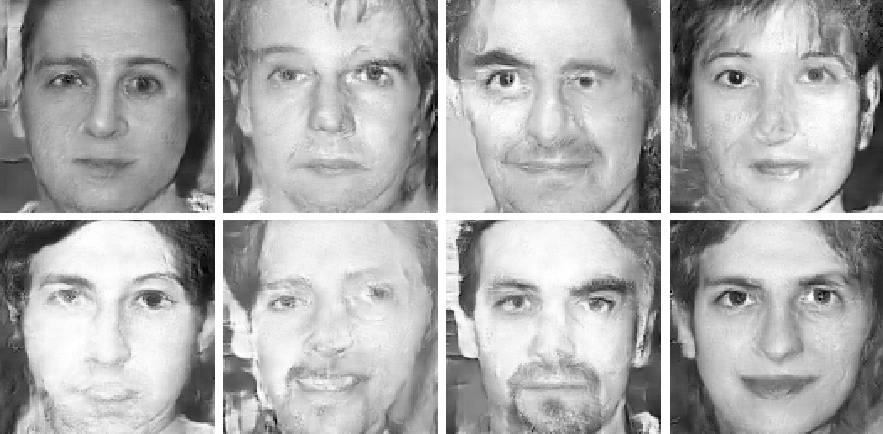
\includegraphics[width=\textwidth]{fig/dcgan/caltech/epoch10000}
        \caption{Epoch 400}
    \end{subfigure}
    \caption{Samples from DCGAN during training on the Caltech dataset}
    \label{dcgan-caltech-samples}
\end{figure}

\begin{figure}

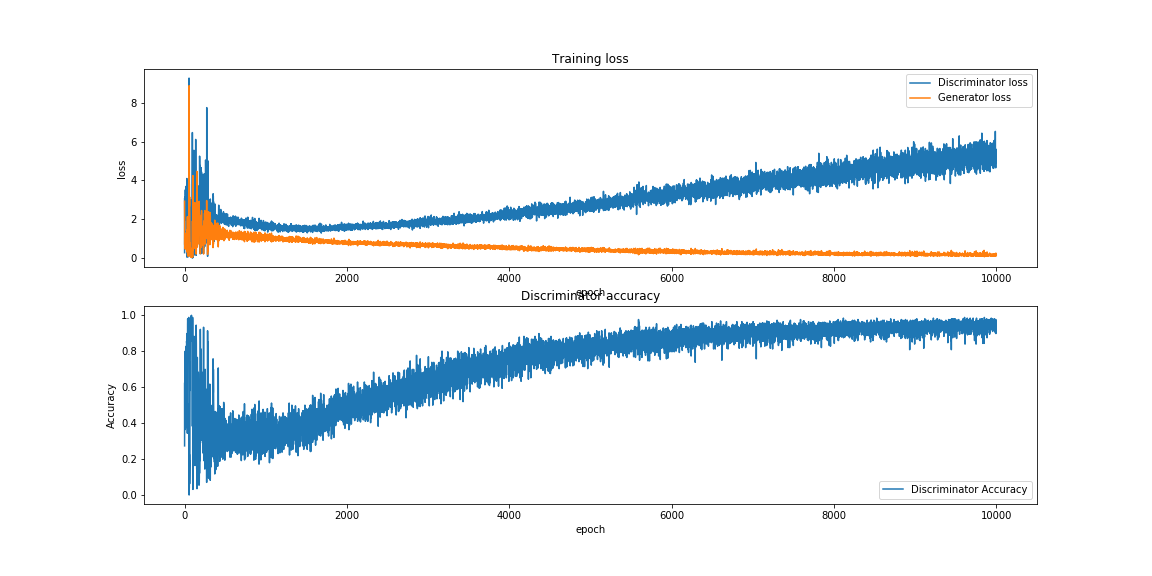
\includegraphics[width=\textwidth]{fig/dcgan/caltech/loss}
  \caption{Loss and accuracy of the discriminator during training on the Caltech Dataset}
  \label{dcgan-caltech-loss}
\end{figure}



% \begin{figure}
%     \centering
%     \begin{subfigure}[b]{0.3\textwidth}
%         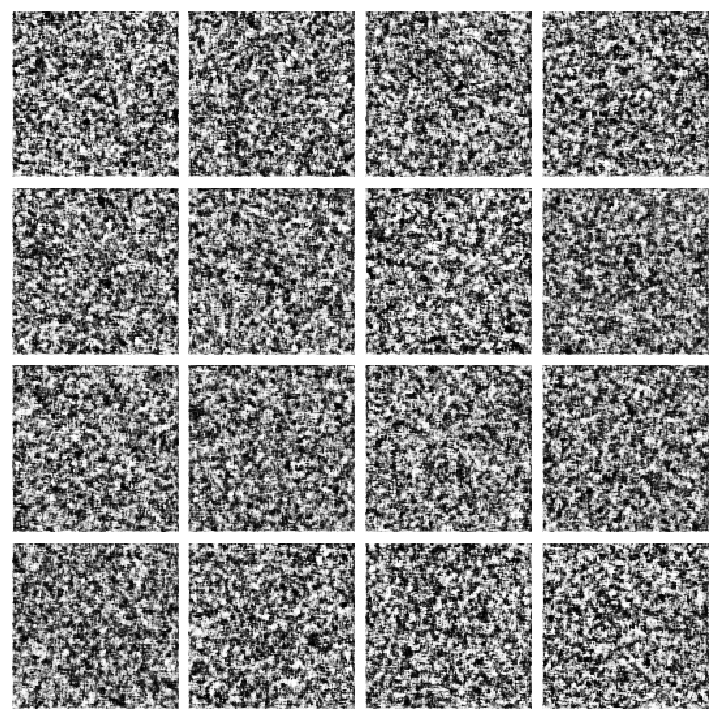
\includegraphics[width=\textwidth]{fig/dcgan/epoch0}
%         \caption{Epoch 0}
%     \end{subfigure}
%     ~
%     \begin{subfigure}[b]{0.3\textwidth}
%         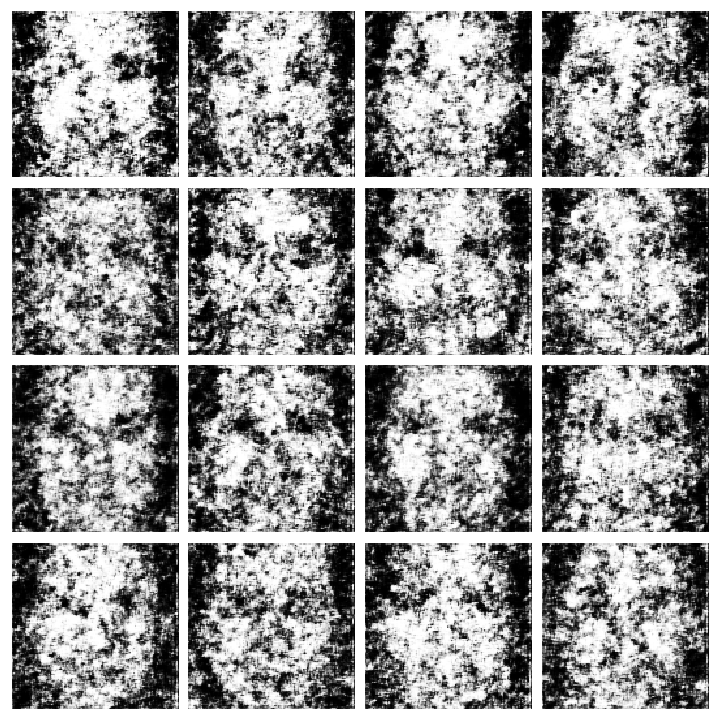
\includegraphics[width=\textwidth]{fig/dcgan/epoch10}
%         \caption{Epoch 10}
%     \end{subfigure}
%     ~
%     \begin{subfigure}[b]{0.3\textwidth}
%         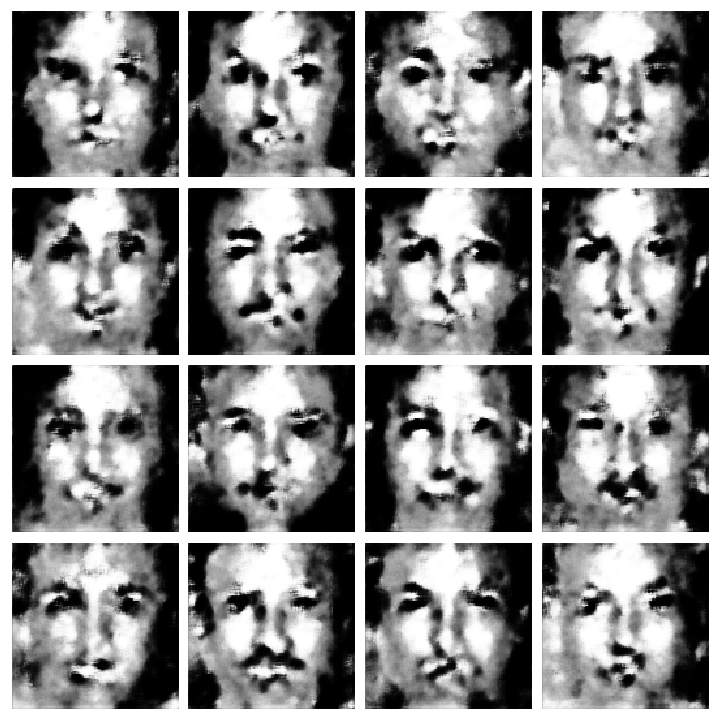
\includegraphics[width=\textwidth]{fig/dcgan/epoch100}
%         \caption{Epoch 100}
%     \end{subfigure}
%
%     \begin{subfigure}[b]{0.3\textwidth}
%         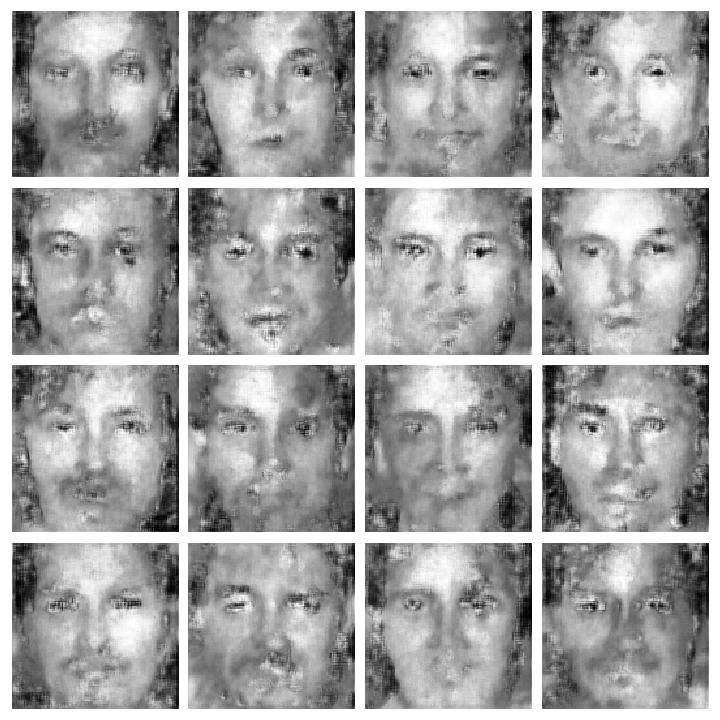
\includegraphics[width=\textwidth]{fig/dcgan/epoch200}
%         \caption{Epoch 200}
%     \end{subfigure}
%     ~
%     \begin{subfigure}[b]{0.3\textwidth}
%         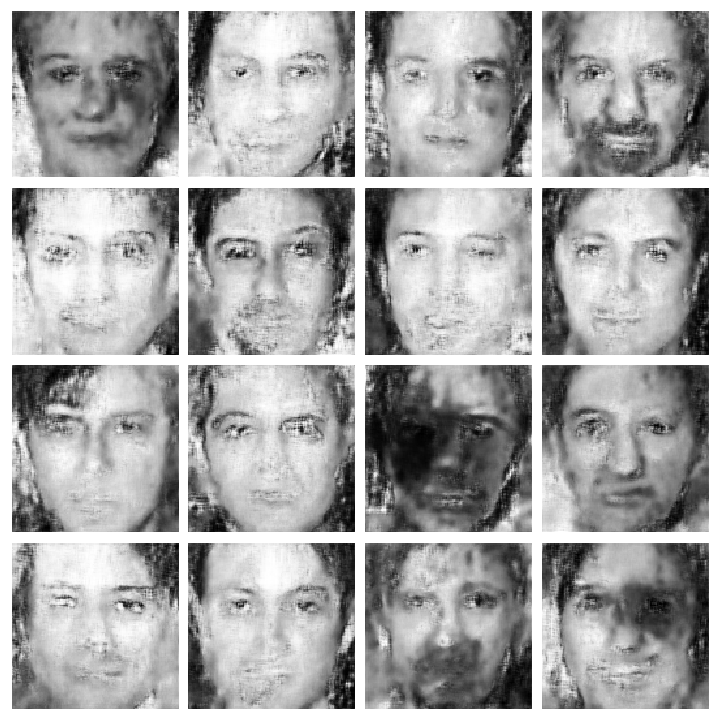
\includegraphics[width=\textwidth]{fig/dcgan/epoch400}
%         \caption{Epoch 400}
%     \end{subfigure}
%     ~
%     \begin{subfigure}[b]{0.3\textwidth}
%         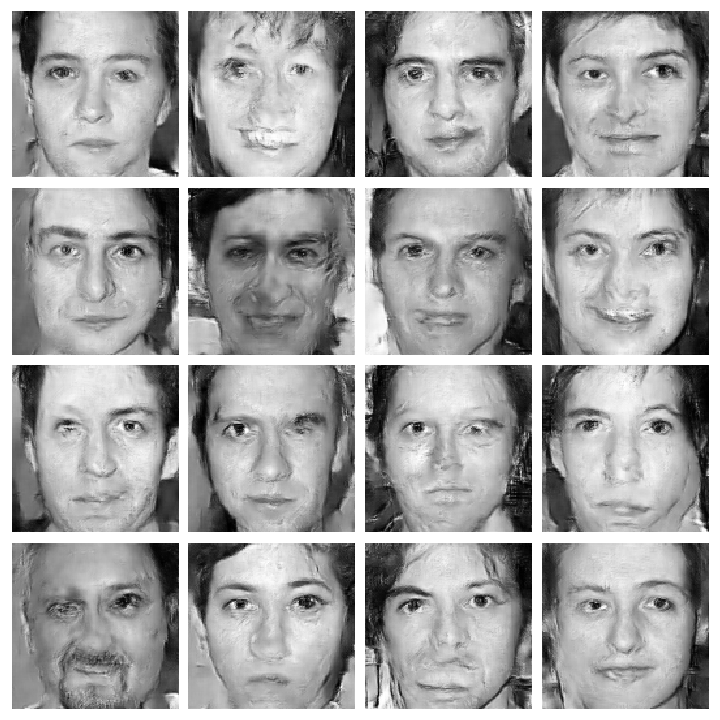
\includegraphics[width=\textwidth]{fig/dcgan/epoch4000}
%         \caption{Epoch 4000}
%     \end{subfigure}
%
%     \caption{Samples from DCGAN during traning on the Caltech dataset}
% \end{figure}

\section{StyleGAN}

We can download the weigths of a pre-trained stylegan trained by Nvidia\footnote{\url{
https://github.com/NVlabs/stylegan.git}}\cite{stylegan}

\begin{figure}
  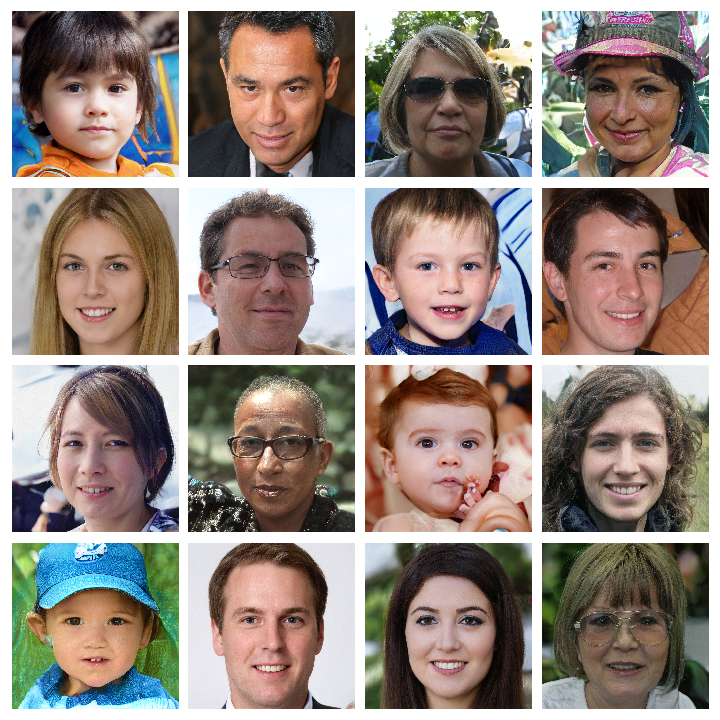
\includegraphics[width=\textwidth]{fig/stylegan/stylegan_example}
  \caption{Random samples from the pretrained StyleGAN}
  \label{StyleGAN-examples}
\end{figure}


\begin{figure}
  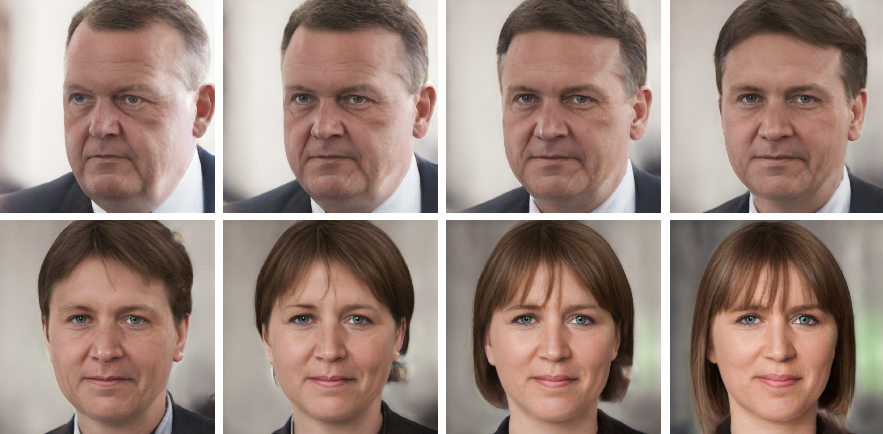
\includegraphics[width=\textwidth]{fig/stylegan/interpolation}
  \caption{Interpolation between two StyleGAN images}
  \label{StyleGAN-interpolation}
\end{figure}


\subsection{Finding the latent space representation of an arbitrary query image.}
Now the pretrained StyleGAN does not contain any encoder network. Therefore there is no way to find a latent space representation of a arbitrary input image.
There is, however a a least two different ways of tackling this problem.
%
% One is the optimization-based
% approach, which directly optimizes the latent code with fixed generator to minimize the pixel-wise reconstruction error [22]. The other is the encoder-based, where an independent encoder network is trained to learn the inverse mapping [37].
\cite{interfacegan}
The paper \textit{Image2StyleGAN: How to Embed Images Into the StyleGAN Latent Space?}\cite{Image2StyleGAN} explicitly investigates this problem.


Here we use the first approach where hold the pretrained generator fixed and then optimize the latent vector to give the desired output image. But instead of calculating the loss directly on the pixel-wise recontruction error.
\footnote{https://github.com/Puzer/stylegan-encoder}



Here we use the same approach as in \cite{styletransfer} where



We use a pre-trained VGG16 network for transforming a query image and the generated image from the latent vector into a high dimensional feature space. The loss is them calculated as a difference between the two feature vectors in the VGG16 feature space.

% Optimization is performed only for latent representation which we want to obtain.

% Upon completion of optimization you are able to transform your latent vector as you wish. For example you can find a "smiling direction" in your latent space, move your latent vector in this direction and transform it back to image using the generator.

%
% \begin{figure}[htb]
%     \centering
%     \begin{subfigure}[b]{\textwidth}
%         \centering
%         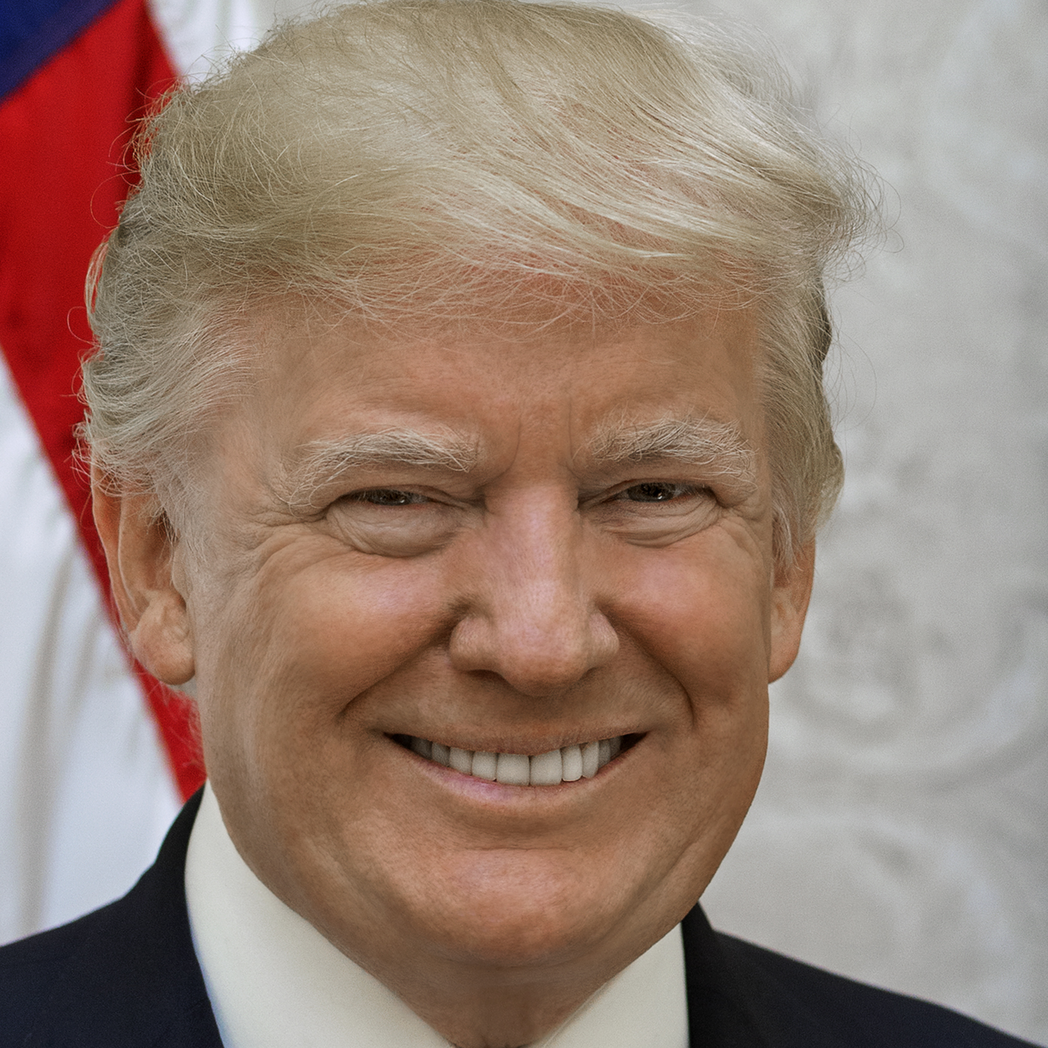
\includegraphics[width=0.3\linewidth]{fig/query_images/trump}%
%         \hfill
%         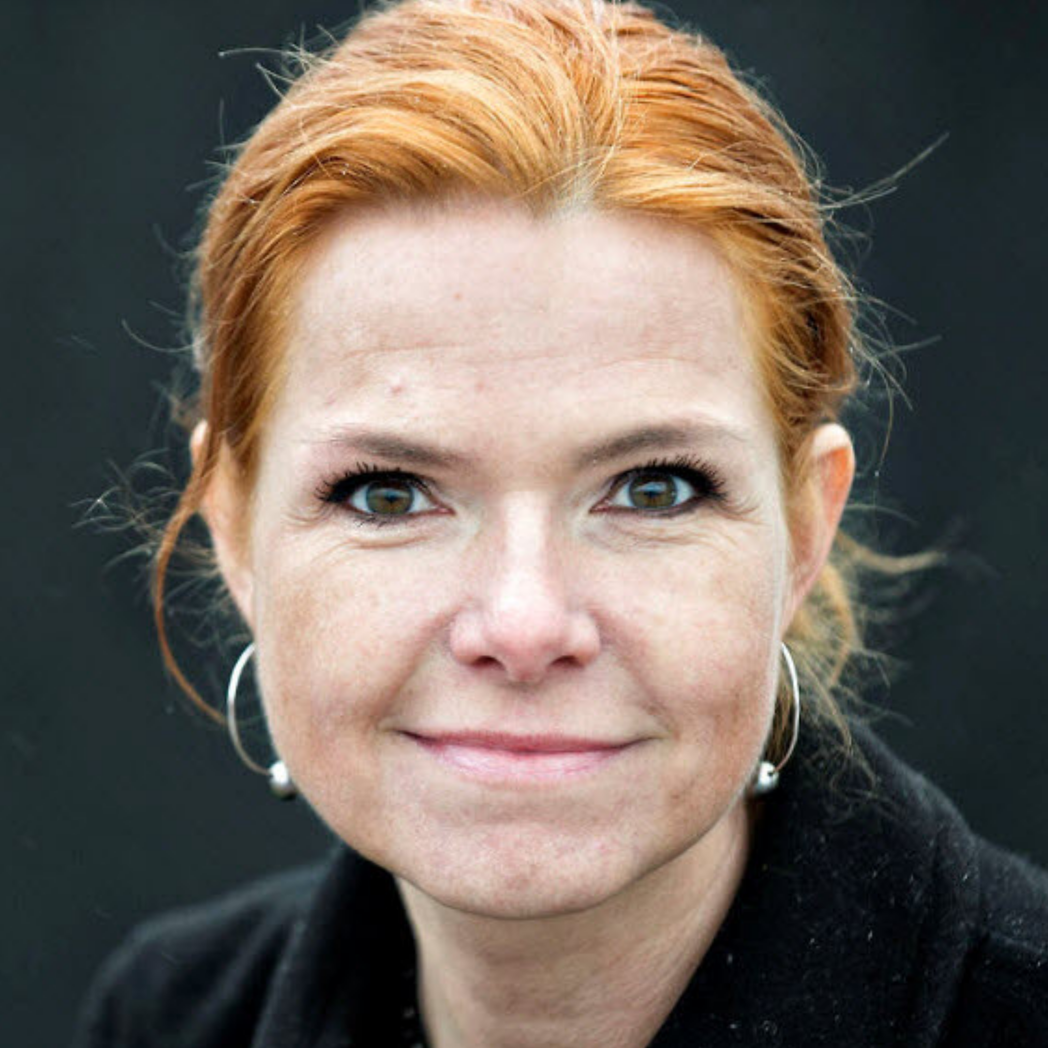
\includegraphics[width=0.3\linewidth]{fig/query_images/inger}
%         \hfill
%         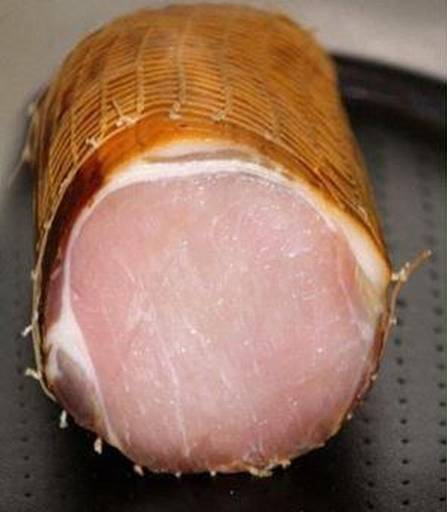
\includegraphics[width=0.3\linewidth]{fig/query_images/skinke}
%         \caption{Original Query Images}
%     \end{subfigure}
%     \vskip\baselineskip
%     \begin{subfigure}[b]{\textwidth}
%         \centering
%         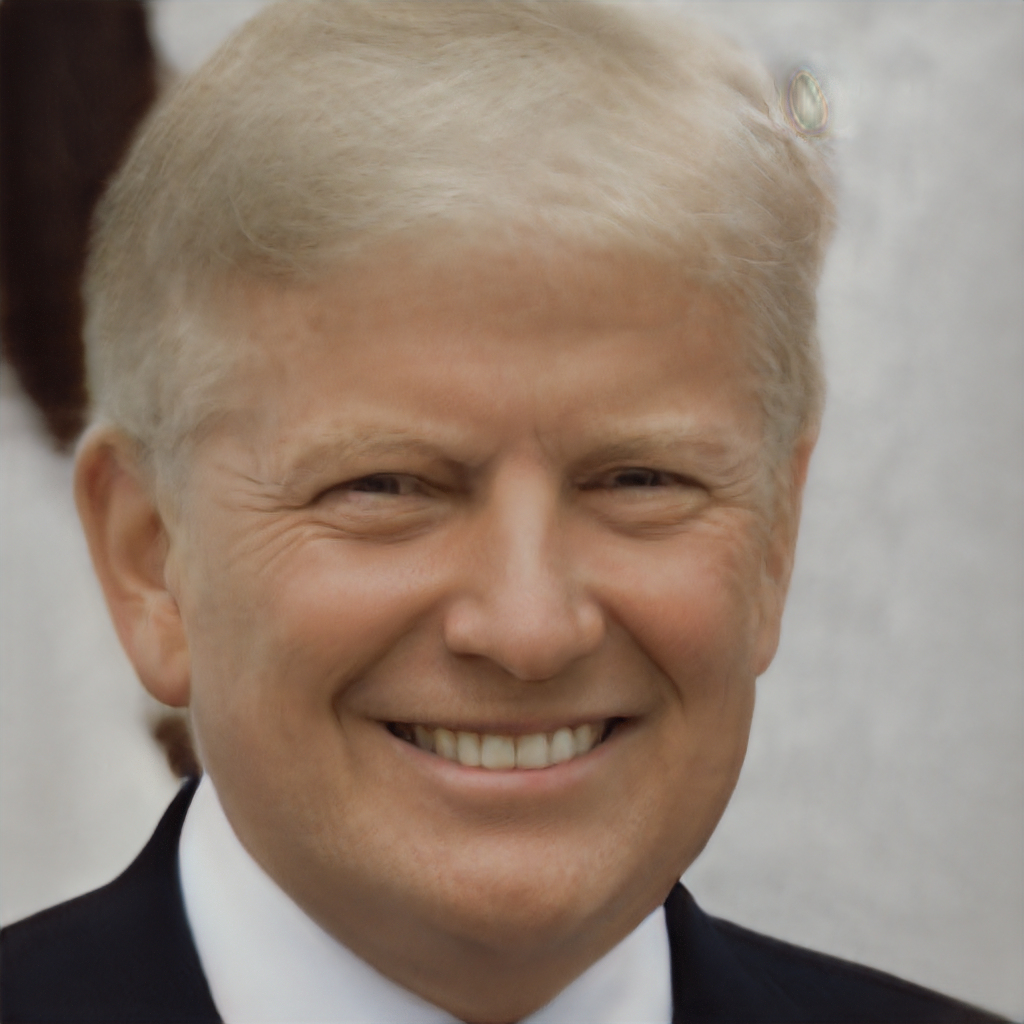
\includegraphics[width=0.3\linewidth]{fig/query_images_reconstucted/trump}%
%         \hfill
%         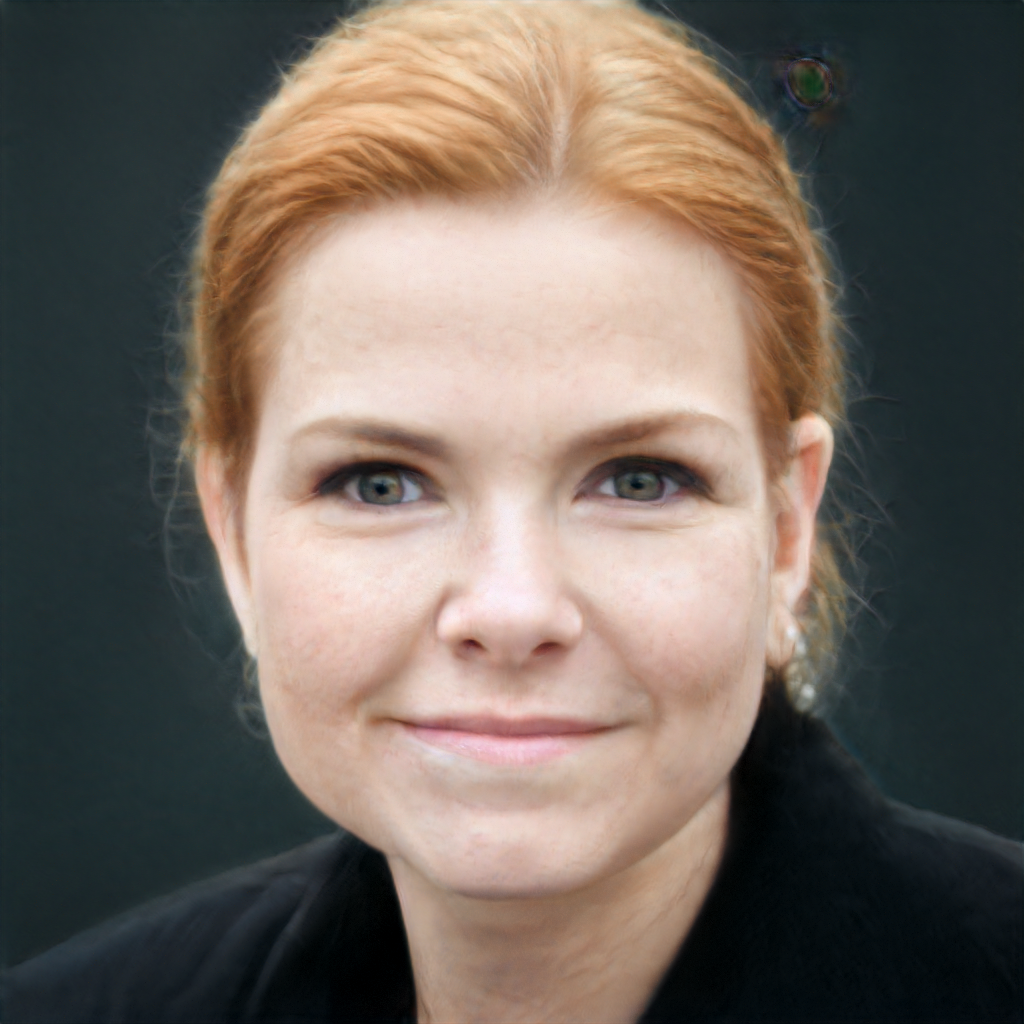
\includegraphics[width=0.3\linewidth]{fig/query_images_reconstucted/inger}
%         \hfill
%         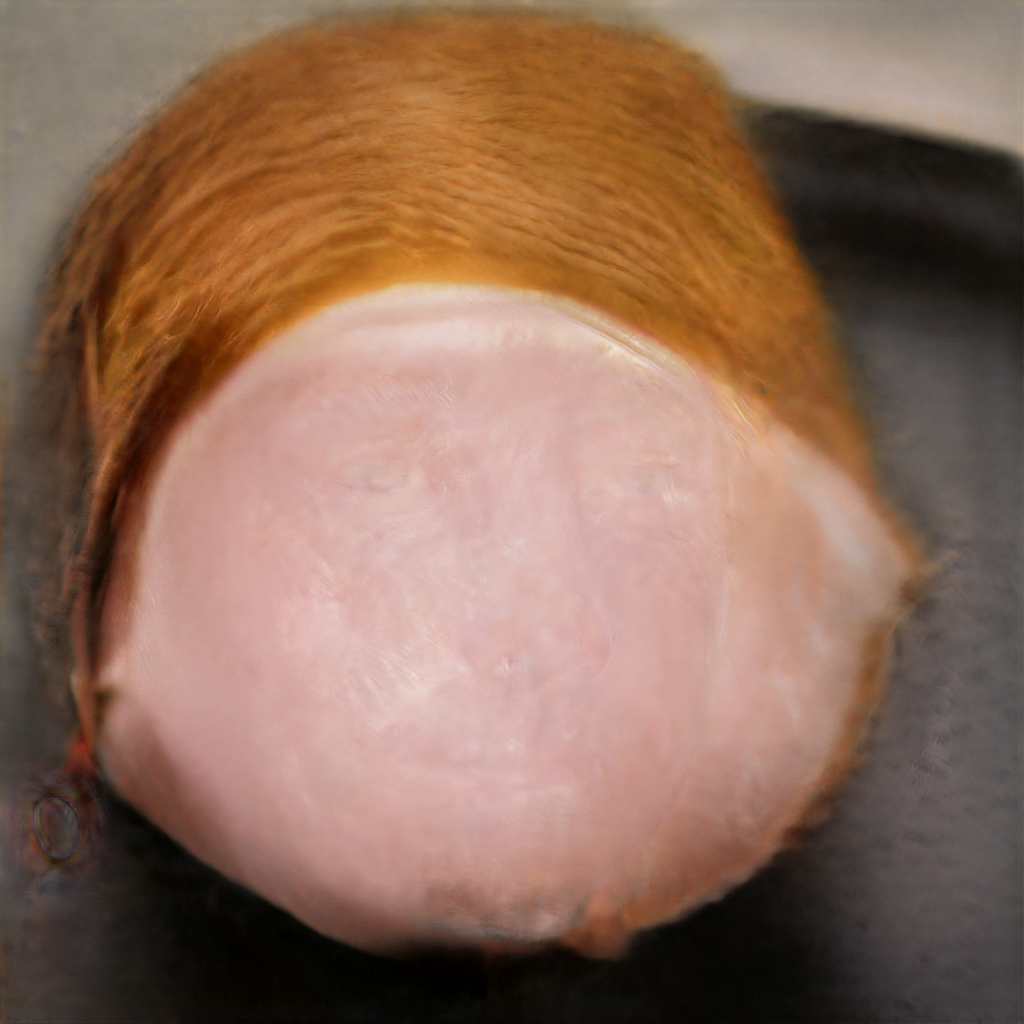
\includegraphics[width=0.3\linewidth]{fig/query_images_reconstucted/skinke}
%         \caption{Reconstructed images from StyleGAN latent space}
%     \end{subfigure}
%     \caption{Latent space representation of arbitrary query images }
% \end{figure}

% \begin{figure}
%     \centering
%     \begin{subfigure}[b]{0.45\textwidth}
%         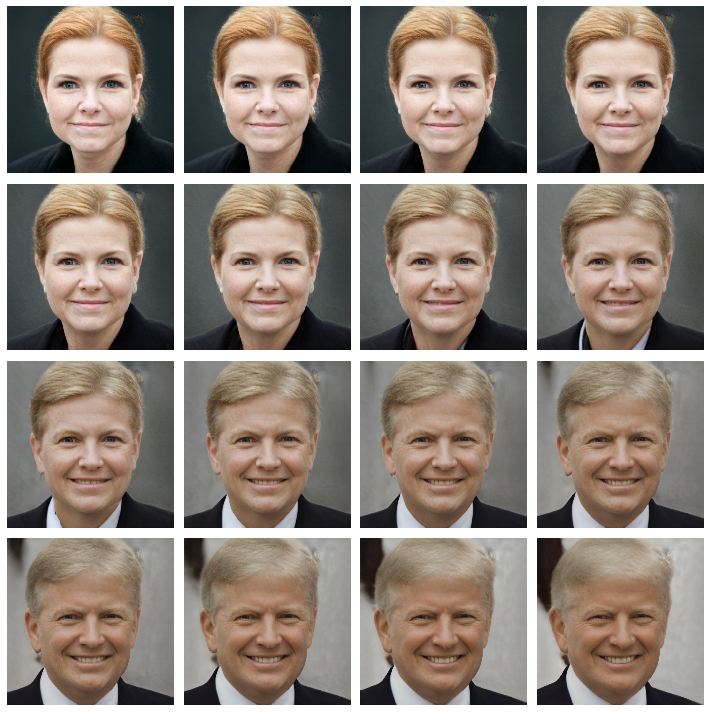
\includegraphics[width=\textwidth]{fig/ingertrump}
%         \caption{Inger Støjberg to Donald Trump}
%     \end{subfigure}
%     ~
%     \begin{subfigure}[b]{0.45\textwidth}
%         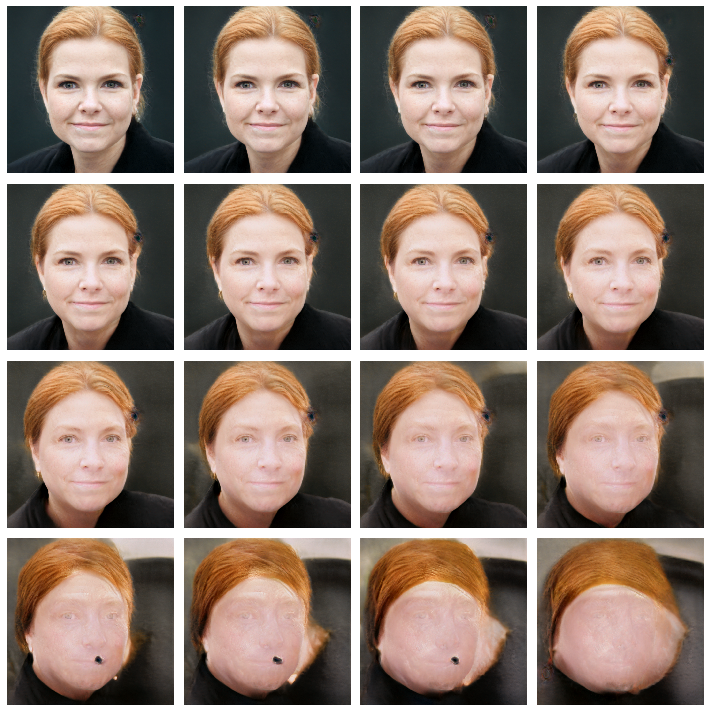
\includegraphics[width=\textwidth]{fig/ingerham}
%         \caption{Inger Støjberg to Ham}
%     \end{subfigure}
%     \caption{Interpolations between query images in the StyleGAN latent space.}
% \end{figure}


\subsection{Semantic face editing.}



\bibliography{references}
\bibliographystyle{plain}

\end{document}
